\documentclass[a4paper, 14pt]{extarticle}
\usepackage[russian]{babel}
\usepackage[T1]{fontenc}
\usepackage{fontspec}
\usepackage{indentfirst}
\usepackage{enumitem}
\usepackage{graphicx}
\usepackage[
  left=20mm,
  right=10mm,
  top=20mm,
  bottom=20mm
]{geometry}
\usepackage{parskip}
\usepackage{titlesec}
\usepackage{xurl}
\usepackage{hyperref}
\usepackage{float}
\usepackage[
  figurename=Рисунок,
  labelsep=endash,
]{caption}
\usepackage[outputdir=build, newfloat]{minted}

\hypersetup{
  colorlinks=true,
  linkcolor=black,
  filecolor=blue,
  urlcolor=blue,
}

\renewcommand*{\labelitemi}{---}
\setmainfont{Times New Roman}
\setmonofont{JetBrains Mono}[
  SizeFeatures={Size=11},
]

\newenvironment{code}{\captionsetup{type=listing}}{}
\SetupFloatingEnvironment{listing}{name=Листинг}

\setminted{
  fontsize=\footnotesize,
  frame=lines,
  framesep=2mm,
}

\setlength{\parskip}{6pt}

\setlength{\parindent}{1cm}
\setlist[itemize]{itemsep=0em,topsep=0em,parsep=0em,partopsep=0em,leftmargin=2.0cm,wide}
\setlist[enumerate]{itemsep=0em,topsep=0em,parsep=0em,partopsep=0em,leftmargin=2.0cm,wide}

\renewcommand{\thesection}{\arabic{section}.}
\renewcommand{\thesubsection}{\thesection\arabic{subsection}.}
\renewcommand{\thesubsubsection}{\thesubsection\arabic{subsubsection}.}

\titleformat{\section}{\normalfont\bfseries}{\thesection}{0.5em}{}
\titleformat{\subsection}{\normalfont\bfseries}{\thesubsection}{0.5em}{}

\titleformat*{\section}{\normalfont\bfseries}
\titleformat*{\subsection}{\normalfont\bfseries}

\linespread{1.5}
\renewcommand{\baselinestretch}{1.5}

\begin{document}

\begin{titlepage}
  \vspace{0pt plus2fill}
  \noindent

  \vspace{0pt plus6fill}
  \begin{center}
    Санкт-Петербургский национальный исследовательский университет
    информационных технологий, механики и оптики

    \vspace{0pt plus3fill}

    Факультет инфокоммуникационных технологий

    Направление подготовки 11.03.02

    \vspace{0pt plus2fill}

    Лабораторная работа №8

    <<Разработка проекта на Django>>

  \end{center}

  \vspace{0pt plus9fill}
  \begin{flushright}
    Выполнил: \\
    Швалов Даниил Андреевич

    Группа: К33211

    Проверила: \\
    Марченко Елена Вадимовна
  \end{flushright}

  \vspace{0pt plus2fill}
  \begin{center}
    Санкт-Петербург

    2023
  \end{center}
\end{titlepage}

\section{Введение}

\textbf{Цель работы}: изучить готовый проект и создать свой проект на Django с
нуля.

\section{Ход работы}

В данной лабораторной работе необходимо создать свой проект на Django, который
будет содержать три страницы: главная, о разработке, страница обратной связи. У
всех трех страниц одинаковые футеры и хидеры.

В ходе разработки приложения было решено в хидер поместить навигационное меню по
сайту. С его помощью пользователь сможет быстро перейти на ту страницу, которая
ему необходима. В футер же, в свою очередь, было принято решение поместить
дополнительную информацию, которая может понадобиться пользователю.

На рис. \ref{fig:index} показана главная страница сайта, которая встречает
пользователя при открытии сайта. На главной странице виден хидер, футер, а также
содержимое самой страницы. В качестве содержимого главной страницы также было
принято решение добавить кнопки для перехода на другие страницы сайта.

\begin{figure}[H]
  \centering
  \fbox{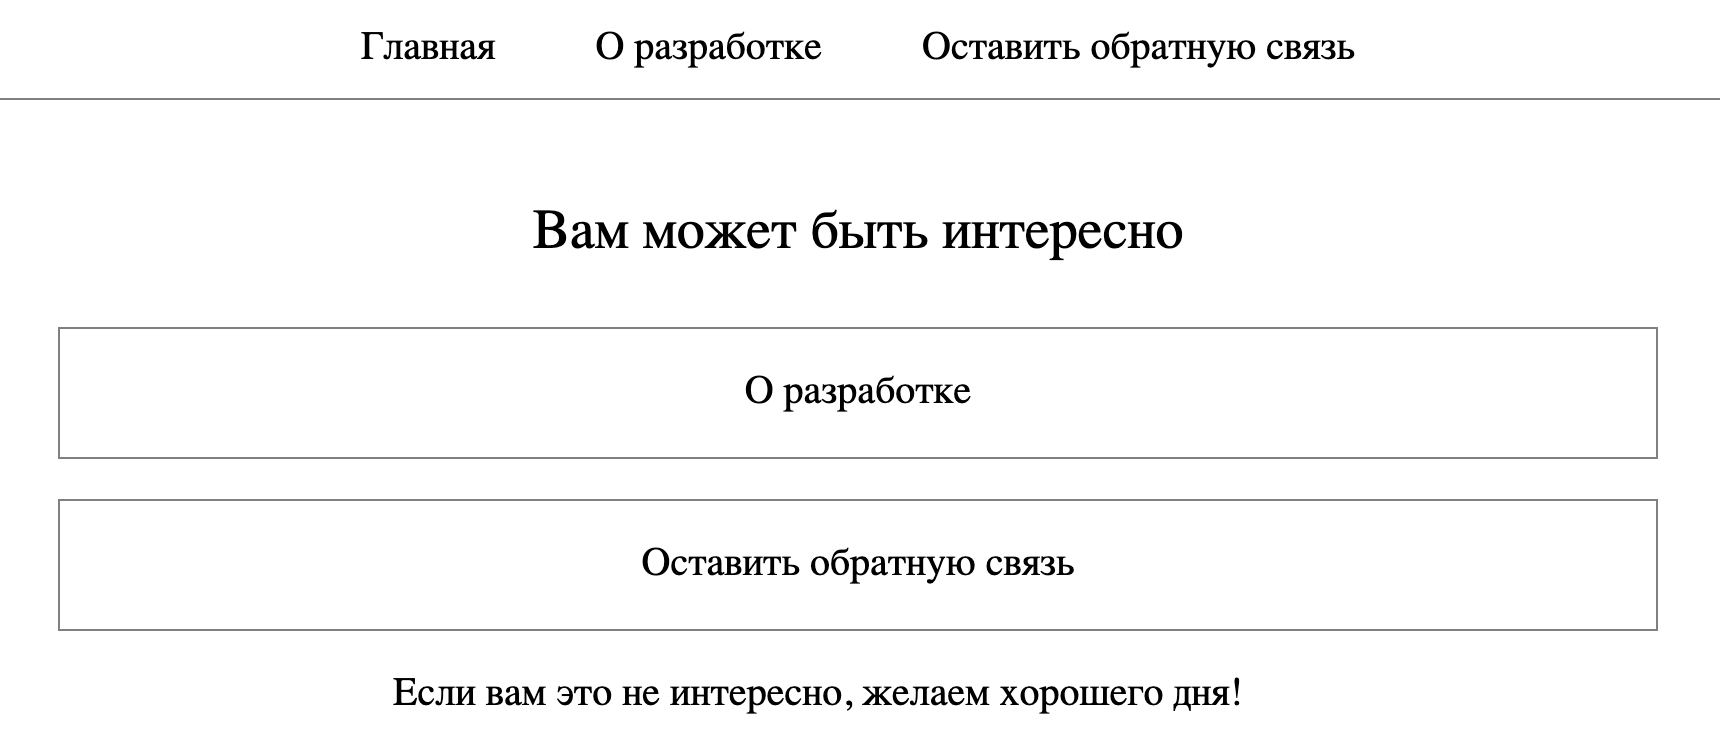
\includegraphics[width=\textwidth]{images/index.png}}
  \caption{Главная страница сайта}
  \label{fig:index}
\end{figure}

При нажатии на кнопку <<О разработке>> открывается страница, показанная на рис.
\ref{fig:about}, которая расположена по относительному адресу \texttt{/about/}.
На данной странице пользователь может узнать больше о приложении и его
устройстве.

\begin{figure}[H]
  \centering
  \fbox{
\includegraphics[width=\textwidth]{images/about.png}}
  \caption{Страница с информацией о разработке}
  \label{fig:about}
\end{figure}

При переходе по кнопке <<Оставить обратную связь>> пользователя перебрасывает на
страницу с формой обратной связи, которая изображена на рис. \ref{fig:feedback}.
Данная страница находится по относительному адресу \texttt{/feedback/}. Здесь
пользователь может оставить свои данные (фамилия, имя, email), оценить качество
обслуживания, отметить, что понравилось больше всего, а также оставить
развернутый комментарий, если это необходимо.

При нажатии на кнопку <<Отправить>> данные отправляются в обработчик по адресу
\texttt{/feedback-submit/}. Там, на стороне бэкенда, данные повторно проверяются
на корректность, после чего сохраняются в базу данных.

Данная форма, а также поля, были взяты из лабораторной работы №3. Логика
проверки и обработки данных была переписана с языка программирования PHP на
Python 3 с использованием фреймворка Django.

\begin{figure}[H]
  \centering
  \fbox{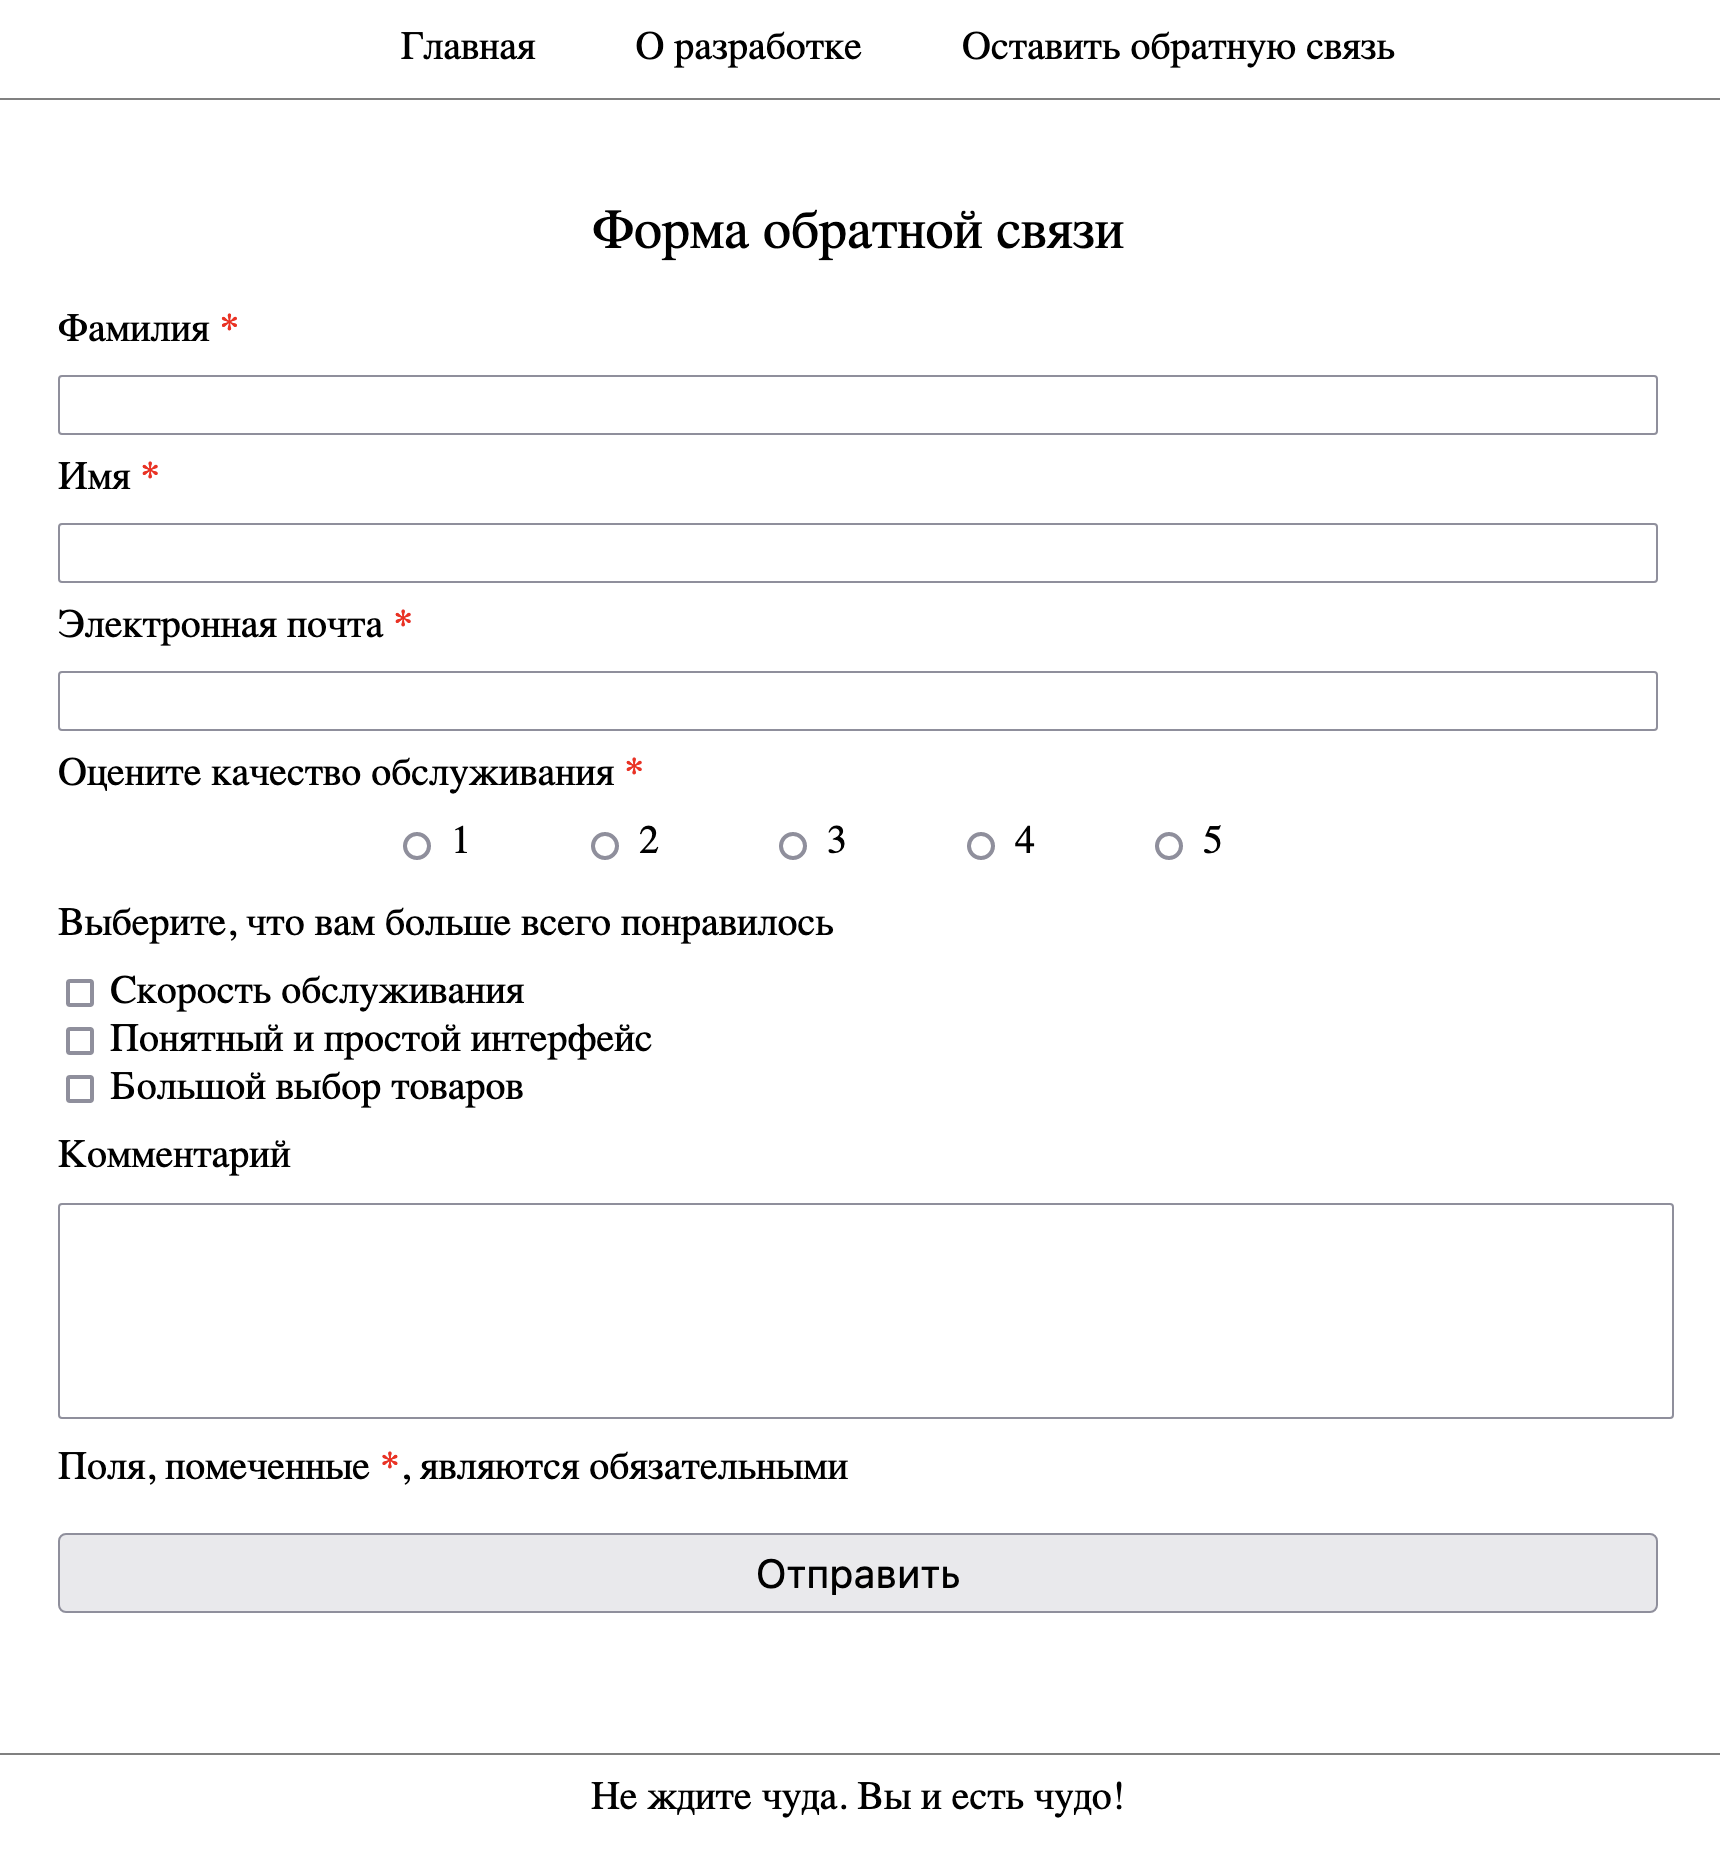
\includegraphics[width=\textwidth]{images/feedback.png}}
  \caption{Страница с формой обратной связи}
  \label{fig:feedback}
\end{figure}

После нажатия кнопки <<Отправить>> и обработки бэкендом полученных данных,
пользователя перебрасывает на страницу с благодарностью за заполнение формы
обратной связи, изображенной на рис. \ref{fig:feedback-success}. На ней
пользователю предлагается вернуться на главную страницу.

\begin{figure}[H]
  \centering
  \fbox{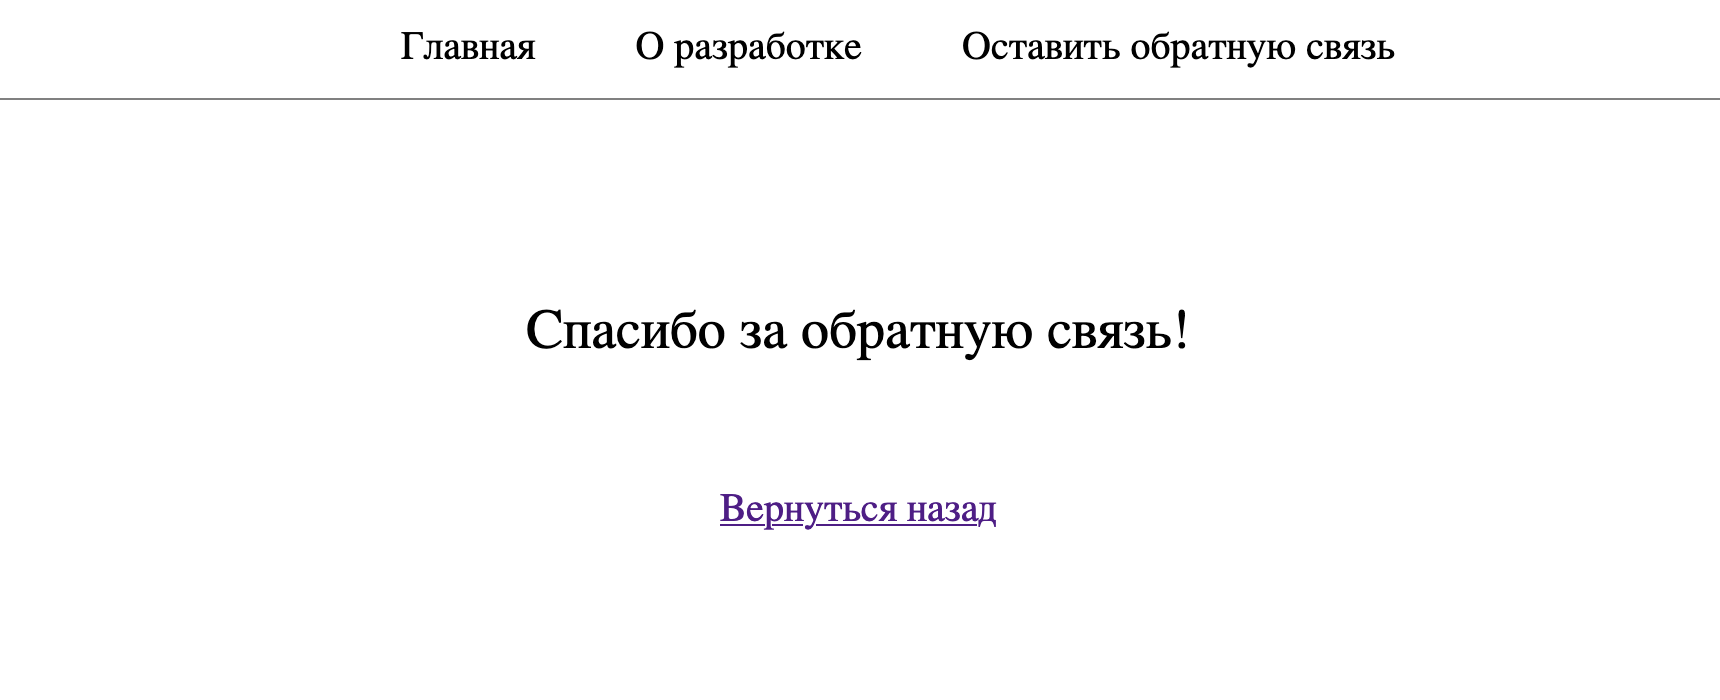
\includegraphics[width=\textwidth]{images/feedback-success.png}}
  \caption{Страница с благодарностью за заполнение обратной связи}
  \label{fig:feedback-success}
\end{figure}

Схема базы данных, в которую сохраняется информация о обратной связи, показана
на рис. \ref{fig:database}. В ней присутствуют все поля, используемые в форме,
т. е. фамилия, имя, электронная почта, качество обслуживания, развернутый
комментарий. Для хранения информации, представленной чек-боксами в форме,
используются булевы поля, значение по умолчанию которых равно \texttt{FALSE}.

\begin{figure}[H]
  \centering
  \fbox{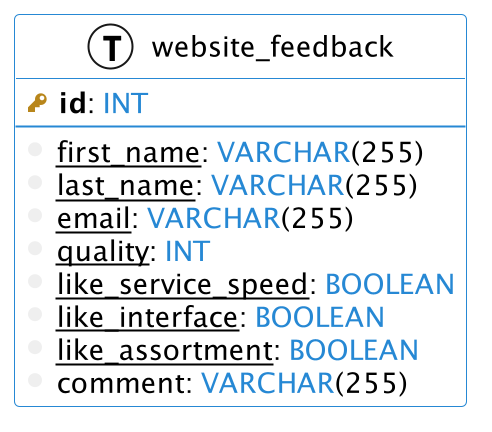
\includegraphics[width=0.4\textwidth]{images/puml/database.png}}
  \caption{Схема базы данных}
  \label{fig:database}
\end{figure}

В качестве СУБД была выбрана СУБД SQLite, поскольку она проста в использовании,
для нее имеется множество документации и обучающих материалов, а также она
хорошо интегрирована в фреймворк Django и не требует дополнительных доработок
для использования основных функций.

Для тестирования работоспособности приложения несколько раз была заполнена форма
обратной связи с различными значениями. На рис. \ref{fig:database-view} с
помощью SQLiteStudio показано содержимое таблицы \texttt{website\_feedback}. Как
видно, бэкенд и СУБД отработали без ошибок и правильно сохранили данные.

\begin{figure}[H]
  \centering
  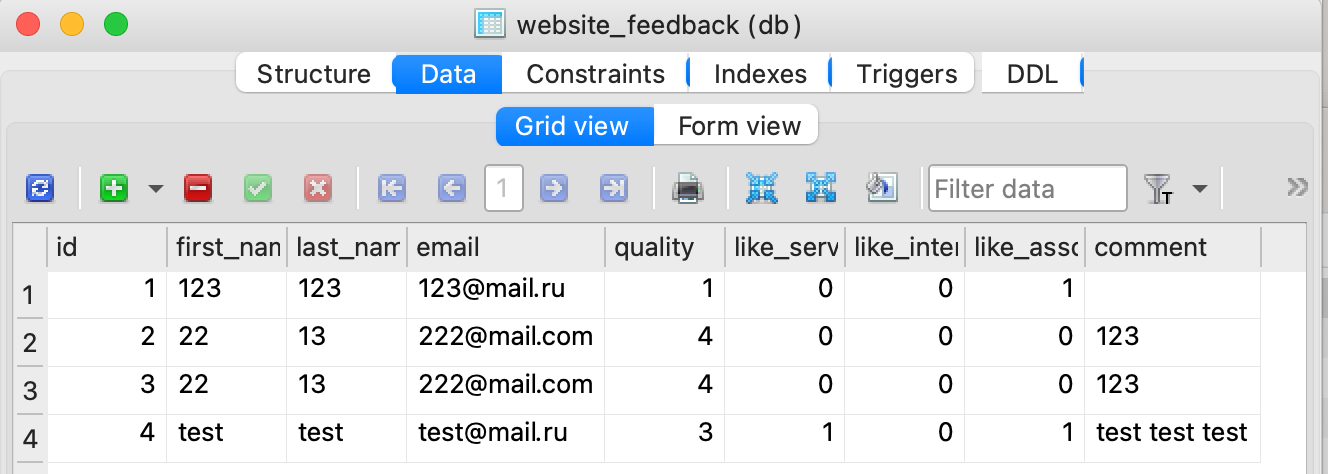
\includegraphics[width=0.8\textwidth]{images/database-view.png}
  \caption{Данные в БД после заполнения нескольких форм обратной связи}
  \label{fig:database-view}
\end{figure}

\section{Вывод}

В ходе выполнения данной лабораторной работы я изучил готовый проект и создал
свой проект на Django с нуля.

\end{document}
